\chapter{Creación del Certificado Personal}

\section{Enunciado}

\textbf{1.1 -- Creación de nuestro certificado personal:}

1.1.1. Leer con mucha atención el apartado ``Generación y verificación de certificados'' de la Wiki ``HowTo
OpenSSL'' (https://openssl.cicei.com). En ese apartado se explica cómo crear un certificado raíz autofirmado
que firma un certificado intermedio y este último firma un certificado final. Comprender todo lo que se explica.

1.1.2.- Entendido el proceso, lo que se nos pide es que utilizando un certificado raíz ya existente y su fichero
de clave (\texttt{certificadoRaiz.cert} y \texttt{certificadoRaiz.key}, disponibles en la página de la asignatura en formato PEM
-- la contraseña de protección de la clave es \texttt{SEGURIDAD}) generemos nuestro certificado personal con los
datos de C, O, OU que se estimen, pero con nuestro nombre y apellidos en CN (common Name) y nuestra
dirección de correo personal en el campo Email Address, los pasos serán:

\begin{itemize}
    \item[a)] Descargar \texttt{certificadoRaiz.crt} y \texttt{certificadoRaiz.key} de la página de la asignatura
    \item[b)] Crear la clave de nuestro certificado (\texttt{openssl genpkey \dots}) $\rightarrow$ \texttt{certificadoPersonal.key}
    (hay que crear una contraseña que protege esta clave -- ANOTARLA)
    \item[c)] Crear el CSR de nuestro certificado (\texttt{openssl req -new \dots}) $\rightarrow$ \texttt{certificadoPersonal.csr}
    \item[d)] Crear nuestro certificado personal a partir del CSR, el certificado raíz y su clave, para ello habrá
    que introducir la contraseña SEGURIDAD que protege la clave de la raíz, el comando será del
    tipo (\texttt{openssl x509 -req -days 365 \dots}) $\rightarrow$ \texttt{certificadoPersonal.crt}
\end{itemize}

Los comandos openssl de los pasos b, c y d están incompletos, pero entendiendo lo que se explica en el apartado
6.2: Certificado intermedio de la Wiki y reemplazando los nombres de ``certificadoIntermedio'' por
``certificadoPersonal'', es fácil de realizar.

Una vez realizados correctamente los pasos anteriores, además del certificado raíz y su clave, tendremos los
ficheros \texttt{certificadoPersonal.key} (protegido con la contraseña que hayan escogido), \texttt{certificadoPersonal.csr}
(ya no nos hace falta, se podría eliminar) y \texttt{certificadoPersonal.crt} (la parte pública de nuestro certificado).

Ya solo nos queda crear un fichero PKCS\#12 con la parte pública y privada de nuestro certificado personal
para poder importarlo en el agente de correo:

\begin{itemize}
    \item[e)] El último apartado de la Wiki, 6.6: PEM a PKCS\#12 explica cómo crear un fichero ``inter.p12'' a
    partir de \texttt{certificadoIntermedio.crt} y \texttt{certificadoIntermedio.key}, tendremos que hacer un comando
    similar, cambiando ``Intermedio'' por ``Personal'' para crear un fichero llamado
    \texttt{certificadoPersonal.p12}. Atención: el comando nos pedirá la clave que protege
    certificadoPersonal y a continuación otra clave (podría ser la misma) para proteger el fichero de
    salida, \texttt{certificadoPersonal.p12}
\end{itemize}

El comando será del tipo (\texttt{openssl pkcs12 export \dots}) $\rightarrow$ \texttt{certificadoPersonal.p12}

\section{Descripción teórica}

Un \textbf{certificado digital X.509} es un documento electrónico que vincula una identidad (nombre, correo electrónico, organización) con una clave pública. Esta vinculación está firmada por una \textbf{Autoridad de Certificación (CA)}, lo que permite a terceros confiar en que esa clave pública pertenece realmente a la identidad indicada.

El proceso de creación de un certificado personal implica los siguientes pasos:

\begin{enumerate}
    \item \textbf{Generar un par de claves} (pública y privada) para el usuario.
    \item \textbf{Crear una solicitud de firma (CSR)}: documento que contiene la clave pública y los datos del solicitante.
    \item \textbf{Firmar el CSR} con el certificado y clave de la CA raíz, generando el certificado final (.crt).
    \item \textbf{Empaquetar en PKCS\#12}: agrupar certificado y clave privada en un único fichero protegido (.p12) para su importación en aplicaciones.
\end{enumerate}

En esta práctica se utiliza un certificado raíz proporcionado por la asignatura (\texttt{certificadoRaiz.crt} y \texttt{certificadoRaiz.key}, protegido con la contraseña \texttt{SEGURIDAD}) como CA que firma nuestro certificado personal.

\section{Paso a) -- Descargar el certificado raíz}

Se descargan los ficheros \texttt{certificadoRaiz.crt} (parte pública) y \texttt{certificadoRaiz.key} (clave privada, protegida con contraseña \texttt{SEGURIDAD}) desde la página de la asignatura y se colocan en el directorio de trabajo.

\section{Paso b) -- Crear la clave del certificado personal}

Se genera una clave privada RSA protegida con cifrado AES-256:

\begin{lstlisting}[caption=Generación de la clave privada del certificado personal]
openssl genpkey -algorithm RSA -out certificadoPersonal.key -aes256
\end{lstlisting}

OpenSSL solicita una contraseña para proteger la clave privada. Esta contraseña será necesaria cada vez que se utilice la clave (por ejemplo, al firmar el CSR o al descifrar mensajes).

\begin{figure}[H]
    \centering
    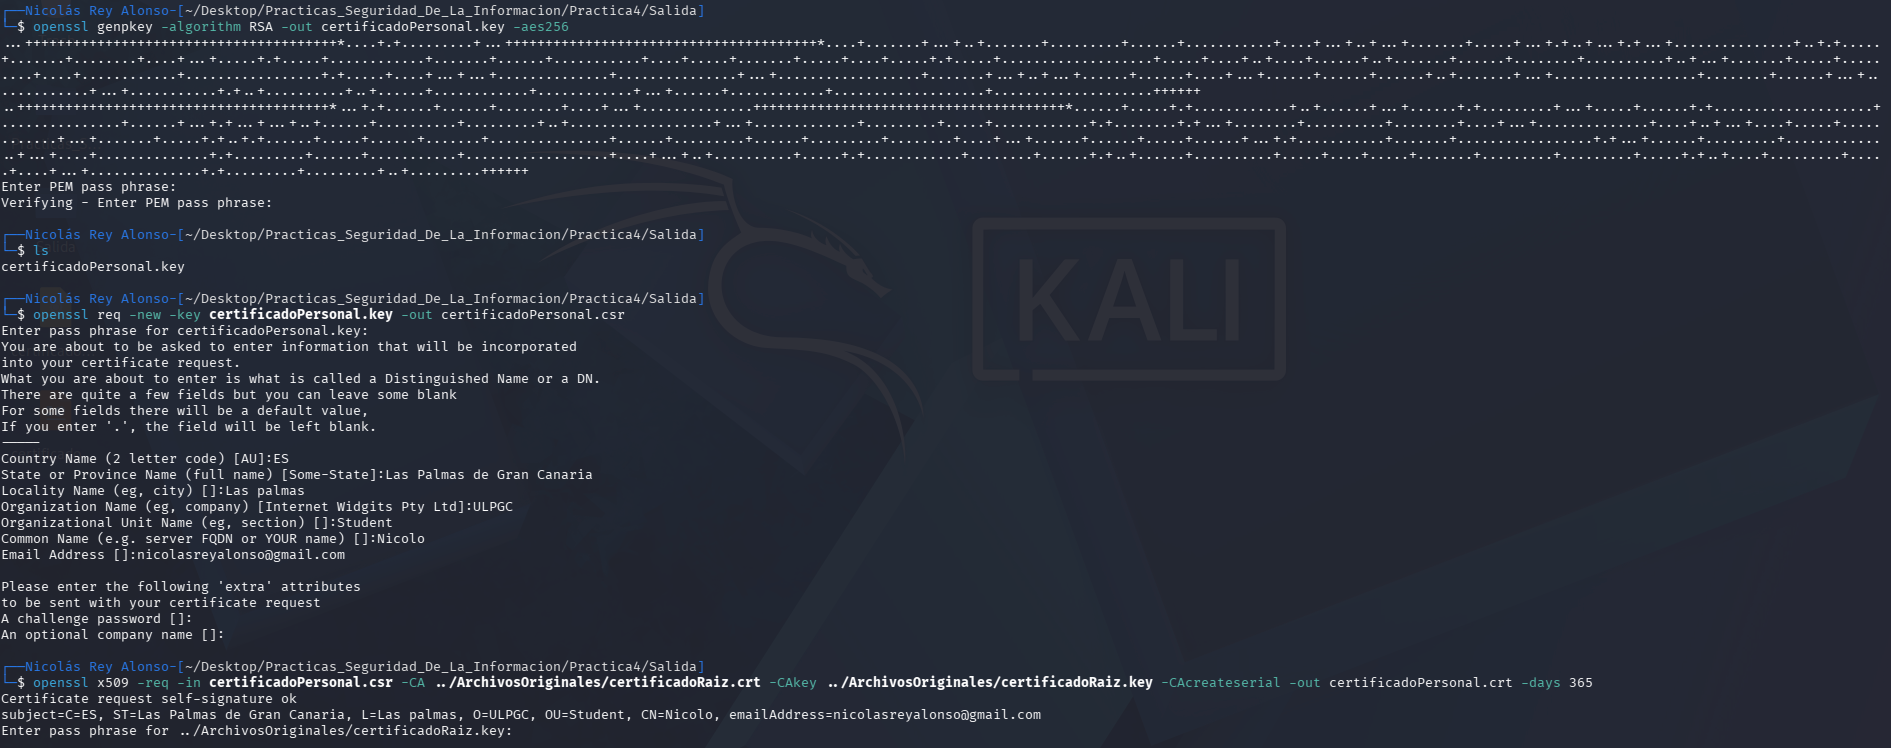
\includegraphics[width=\textwidth]{Imagenes/1.1.1.png}
    \caption{Generación de la clave personal y creación del CSR en terminal}
    \label{fig:creacion_clave_csr}
\end{figure}

\section{Paso c) -- Crear el CSR (Certificate Signing Request)}

El CSR incluye la clave pública y los datos identificativos del solicitante (país, organización, nombre, correo):

\begin{lstlisting}[caption=Creación del CSR]
openssl req -new -key certificadoPersonal.key -out certificadoPersonal.csr
\end{lstlisting}

Durante el proceso se introducen los campos del certificado:

\begin{itemize}[label=\textbullet]
    \item \textbf{C} (Country): ES
    \item \textbf{O} (Organization): ULPGC -- Seguridad de la Información
    \item \textbf{OU} (Organizational Unit): EII
    \item \textbf{CN} (Common Name): Nicolás Rey Alonso
    \item \textbf{Email}: dirección de correo personal
\end{itemize}

\section{Paso d) -- Firmar el CSR con el certificado raíz}

Se firma el CSR utilizando el certificado raíz y su clave privada, generando nuestro certificado personal con validez de 365 días:

\begin{lstlisting}[caption=Firma del CSR con el certificado raíz]
openssl x509 -req -in certificadoPersonal.csr \
    -CA certificadoRaiz.crt -CAkey certificadoRaiz.key \
    -CAcreateserial -out certificadoPersonal.crt -days 365
\end{lstlisting}

Se introduce la contraseña \texttt{SEGURIDAD} que protege \texttt{certificadoRaiz.key}. El resultado es el fichero \texttt{certificadoPersonal.crt} que contiene nuestra clave pública firmada por la CA raíz.

\begin{figure}[H]
    \centering
    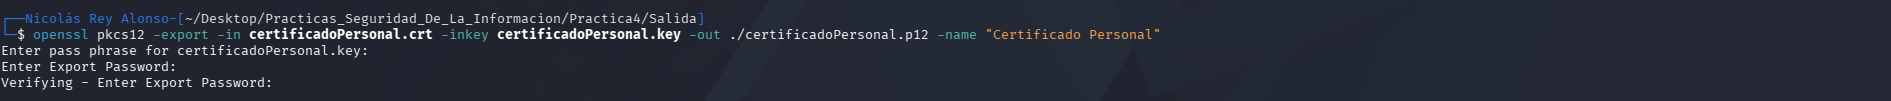
\includegraphics[width=\textwidth]{Imagenes/1.1.2.png}
    \caption{Firma del CSR y creación del fichero PKCS\#12}
    \label{fig:firma_csr_p12}
\end{figure}

\section{Paso e) -- Crear el fichero PKCS\#12}

El formato PKCS\#12 (.p12) empaqueta el certificado personal y la clave privada en un único fichero protegido con contraseña, adecuado para importar en clientes de correo como Thunderbird:

\begin{lstlisting}[caption=Creación del fichero PKCS\#12]
openssl pkcs12 -export -in certificadoPersonal.crt \
    -inkey certificadoPersonal.key \
    -out certificadoPersonal.p12 -name "Certificado Personal"
\end{lstlisting}

El comando solicita:
\begin{enumerate}
    \item La contraseña de \texttt{certificadoPersonal.key} (la que creamos en el paso b).
    \item Una nueva contraseña de exportación para proteger el fichero \texttt{.p12}.
\end{enumerate}

\section{Ficheros resultantes}

Tras completar el proceso, se dispone de los siguientes ficheros:

\begin{table}[H]
    \centering
    \caption{Ficheros generados en la creación del certificado}
    \begin{tabularx}{\textwidth}{l|l|X}
        \toprule
        \textbf{Fichero} & \textbf{Formato} & \textbf{Contenido} \\
        \midrule
        certificadoPersonal.key & PEM & Clave privada RSA cifrada con AES-256 \\
        certificadoPersonal.crt & PEM & Certificado personal (clave pública firmada por la CA) \\
        certificadoPersonal.p12 & PKCS\#12 & Clave privada + certificado en un solo fichero \\
        \bottomrule
    \end{tabularx}
\end{table}

El fichero \texttt{certificadoPersonal.csr} se elimina tras la firma, ya que no es necesario conservarlo.
